\documentclass[a4paper]{report}
\usepackage[english]{babel}
\usepackage{caption}
\usepackage{subcaption}
\usepackage{listings, color}
\usepackage{graphicx}
\usepackage{chngpage}
\usepackage{longtable}
\usepackage{float}
\usepackage{comment}
\usepackage[usenames,dvipsnames]{xcolor}
\usepackage{epstopdf}
\usepackage{titlesec}
\usepackage{pdfpages}
\usepackage{wrapfig}
\usepackage{url}
\usepackage{hyperref}
\usepackage[nodisplayskipstretch]{setspace}
\usepackage[top=2cm,bottom=2.5cm]{geometry}
\usepackage{amsmath}
\usepackage{caption} 
\usepackage{natbib}
\usepackage[nottoc,numbib]{tocbibind}
\usepackage{xpatch}

\definecolor{dkgreen}{rgb}{0,0.6,0}
\definecolor{gray}{rgb}{0.5,0.5,0.5}
\definecolor{mauve}{rgb}{0.58,0,0.82}

\setlength{\parindent}{0pt}

\lstset{frame=tb,
  language=Matlab,
  aboveskip=3mm,
  belowskip=3mm,
  showstringspaces=false,
  columns=flexible,
  basicstyle={\small\ttfamily},
  numbers=left,
  numberstyle=\tiny\color{gray},
  keywordstyle=\color{black},
  commentstyle=\color{dkgreen},
  stringstyle=\color{mauve},
  breaklines=true,
  breakatwhitespace=true
  tabsize=3
}

\newcommand{\tab}{\hspace*{2em}}
\titleformat{\chapter}{\normalfont\huge\bf}{\thechapter.}{20pt}{\huge\bf}

\newcommand\fnurl[2]{%
  \href{#2}{#1}\footnote{\url{#2}}%
}


\xpatchcmd{\itemize}
  {\def\makelabel}
  {\setlength{\itemsep}{0em}\def\makelabel}
  {}
  {}

\begin{document} 
\begin{titlepage}

\newcommand{\HRule}{\rule{\linewidth}{0.5mm}} % Defines a new command for the horizontal lines, change thickness here

\center % Center everything on the page
 
%----------------------------------------------------------------------------------------
%	HEADING SECTIONS
%----------------------------------------------------------------------------------------

\textsc{\LARGE Group 7}\\[1.5cm] % Name of your university/college

%----------------------------------------------------------------------------------------
%	TITLE SECTION
%----------------------------------------------------------------------------------------

\HRule \\[0.4cm]
{ \huge \bfseries Assignment 3}\\[0.4cm] % Title of your document
\HRule \\[4cm]
 
%----------------------------------------------------------------------------------------
%	AUTHOR SECTION
%----------------------------------------------------------------------------------------

\begin{minipage}{0.5\textwidth}
\emph{Authors:}\\     
Emilie de Bree - 4247558\\
Toine Hartman - 4305655\\
Jeffrey Helgers - 4318749 \\
Jim Hommes - 4306090\\
Joost Pluim - 4162269 \\
Matthijs Verzijl - 4282604\\\\
\emph{Supervisor:} \\
Alberto Bacchelli \\\\
\emph{Teaching Assistant:} \\
Aaron Ang\\
\end{minipage}\\[4cm]


%----------------------------------------------------------------------------------------
%	LOGO SECTION
%----------------------------------------------------------------------------------------


\includegraphics[width=100mm]{logo.jpg}\\[1cm] % Include a department/university logo - this will require the graphicx package

%----------------------------------------------------------------------------------------
%	DATE SECTION
%----------------------------------------------------------------------------------------

{\large \today}\\[3cm] % Date, change the \today to a set date if you want to be precise

\vfill % Fill the rest of the page with whitespace

\end{titlepage}
\tableofcontents
\thispagestyle{empty}
\setcounter{page}{0}
\chapter{20-Time, Revolutions}

\section{Question 1}

In this sprint, we wanted to add 3 main new features. The first was the ability to add a high score. The idea behind this was that the scores could be kept and seen again, and that there would be a high score screen to show what the top scores for the game were. The second feature was the ability to have options, so that for example the music could be turned off by the player, if they do not like it. The final thing we wanted to add to our game, was a boss. The boss has to have the ability to shoot the player. To make this boss harder to kill we gave the boss a few lives. Now when you have completed all the normal levels, the boss level appears, and when you kill the boss you win the game.

\section{Question 2}

\subsection{Introduction}

For the boss, two new classes had to be add, 'FinalEnemy' and 'BubbleEnemy', both these classes are related to other classes.

\subsection{Responsibility Driven Design} 

\subsubsection{FinalEnemy}
\textit{Responsibility:} \\
The final enemy has to be able to move from the top to the bottom of the screen, and it has to be able to shoot a BubbleEnemy. When the player hits the final enemy with it's bubble, he has to lose a life. \\ \\
\textit{Collaborations:} \\
FinalEnemy collaborates with Observable to be able to send updates to Observer classes. It also collaborates with  the SpriteBase, to get the x and y, and with both the Bubble extendsions, to fire bubbles and to be shot by bubbles.

\subsubsection{BubbleEnemy}
\textit{Responsibility:} \\
The BubbleEmey's are shot by the FinalEnemy, these bubbles have the ability to move through walls. When one of these bubbles hits the player, the player has to die. \\ \\
\textit{Collaborations:} \\
BubbleEnemy collaborates with Observable to be able to send updates to Observer classes. It also collaborates with  the SpriteBase, to get the x and y, with the FinalEnemy to be shot by, and with the Player to kill.

\subsubsection{Highscore}
\textit{Responsibility:} \\
The StartController asks the name(s) of the player(s) via the NameInputController. The highscores are build up of HighscoreEntryControllers, which gets and sets the scores in Settings. \\ \\
\textit{Collaborations:} \\
StartController collaborates with NameInput and HighscoreEntryController to manage custom player names for the highscores. HighscoreEntryController collaborates with Settings to save and retrieve the highscores so they are saved even after the game is stopped.

\subsection{UML}

\subsubsection{Highscore}

The followg UML is for the High Score feature.
\\\\
\includegraphics[width=150mm]{HighscoreUML.png}

\subsubsection{Options}

\subsubsection{Final Boss}

The following UML is the UML for the Boss feature.
\\\\
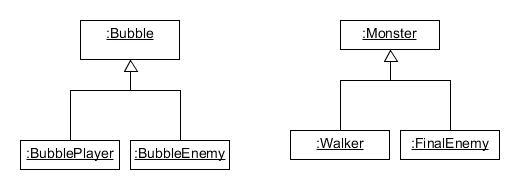
\includegraphics[width=150mm]{FinalEnemyUml.png}




\chapter{Design patterns}

\section{Model View Controller}

\subsection{MVC Description}
The MVC is implemented by using JavaFX. If you look at the figure below, you see the principle of the MVC design pattern. The model is loaded by creating a Stage with a FXML file as resource. The Stage is the View for the user and the FXML file also creates a designated controller (MainController, StartController and GameEndController). The View properties can be loaded using @FXML tags. Now, when the user interacts, the information is sent to the designated controller that in turn sents the information to the View. In reality, it's more like the figure below.
\\\\
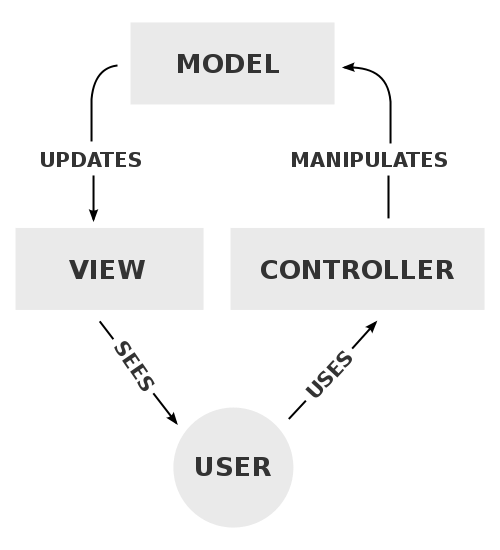
\includegraphics[width=80mm]{MVC.png}

\subsection{MVC Class Diagram}

Below is the class diagram of the Model View Controller design pattern, as found in our code.
\\\\
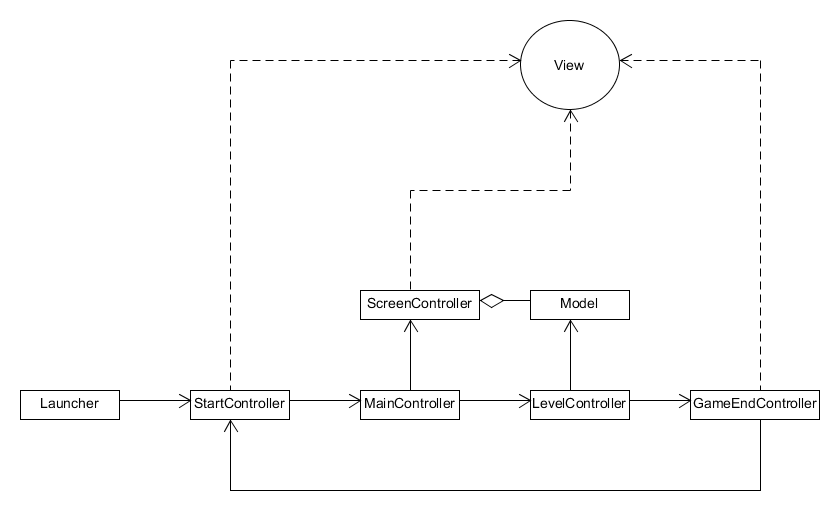
\includegraphics[width=150mm]{UML_MVC.png}

\subsection{MVC Sequence Diagram}

Below is the sequence diagram of the Model View Controller design pattern, as found in our code.
\\\\
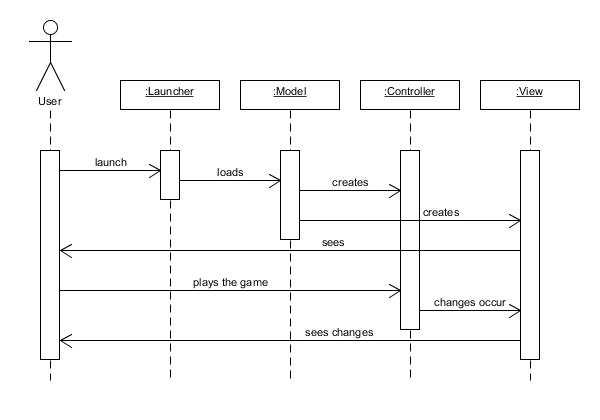
\includegraphics[width=150mm]{MVC_sequence.jpg}
\section{Design Pattern 2}

\subsection{Description Design Pattern 2}
`Write a natural language description of why and how the pattern is implemented in your code.'

\subsection{Class Diagram Design Pattern 2}
`Make a class diagram of how the pattern is structured statically in your code.'

\subsection{Sequence Diagram Design Pattern 2}
`Make a sequence diagram of how the pattern works dynamically in your code'
\chapter{Wrap up: Reflection}

\section{Essay}
The course Software Engineering Methods involved the learning of engineering methods, tactics of working in a group, coping with deadlines and because of the latter: planning. But most of all it was a great experience, and gave us the chance to learn new Software Engineering Methods. By first being told to make a game within 2 weeks, and afterwards by implementing information heard in lectures, it was a journey of learning by doing. When doing this, we of course experienced different bumps in the road, but all of these made us a better and more experienced group, more efficient and eventually allowed us to made a better game. We will take you through our journey by highlighting a couple aspects:

\subsection{Code quality}
When going back to our initial product, we of course see that the product was lacking features, and was therefore not as much fun to play as it is now. But moreover, we see that our code quality has improved drastically. Implementing for example Design Patterns at first sounded unnecessary, time-consuming and above all irrelevant. However when learning about these patterns and once implementing them, we started to realise that they could be useful. Once the design patterns were actually implemented it became obvious that the code was improving, and that these design patterns were actually really helpful. They provided a basis for easily adding new features or extending already existing features. Therefore they were in fact very useful in extending and improving our game. Looking back, it would have been better if we could have implemented these design patterns earlier, but that is of course all a part of the learning curve. 

\subsection{Teamwork}
At the start of the project, some of the team members were more experienced than others with working in teams on software projects. So at the start of the project the ones with more experience took the lead in setting up the project. However, the others quickly were able to keep up, once familiar with the work flow. This however didn't mean that \fnurl{Parkinson's Law}{https://en.wikipedia.org/wiki/Parkinson\%27s_law} was always applied to our project, especially in the first few sprints. A deadline on Friday night often meant a busy Friday night coding. This was however taken into account in every Sprint Reflection, and we learnt from our mistakes, which means that nowadays the work is more evenly spread over the week. A nice benefit is a more relaxed Friday nights with an in-time delivery of the game. While advancing through this period we also clearly became more confident in telling each other what the good and especially the bad practices of delivered Pull Requests were. This made the team work a lot more efficient than in the beginning of the project. A big benefit above all was that our group included a couple good `managers' who were able to divide all tasks every Tuesday very clearly so that everyone knew what he or she was up to that week. Every team member took the tasks they thought they were good in, or the task with techniques they wanted to learn more about. Good support by other team members always lead to a good improvement of the game every Friday. 

\subsection{Reviewing}
An important part of our learning process in this subject was learning the way code is being reviewed in a game. Not everyone was familiar with a good GitHub work flow, with the reviewing of Pull Requests, but once advancing through this learning period, the reviewing process speeded up, allowing the reviewing to become more efficient. We all became sharper at the things to look at, and while maybe in the beginning some of the times only the game and tests were run, after a while good code advices and improvements were suggested and maven was always run. This also lead to a better game which, behind the scenes also ran better and functioned better. Especially when introducing the `Software Metrics', quite interesting aspects and quite important improvements became clear. This definitely fulfilled an important role to show for example the fact that we had created a few God classes, which needed to change.  

\subsection{Testing}
Although testing is of course an important part of the game, always fully complying with a completely test-driven development still is a hard thing to implement in reality. In theory of course this is the best way to go, but in reality we learned that it was often more convenient to first write code and afterwards write the tests for the just implemented features. On the other hand we did manage to divide features in small enough parts so that we didn't have to write huge amounts of code and write the belonging tests afterwards. This meant that small parts of code were quickly followed by tests to make sure the feature worked as it was supposed to. \\
Sometimes we did experience that having bigger features, often lead to branches being open for a longer period of time. This in its turn led to merge conflicts once the feature was submitted as a Pull Request. In the beginning of the project this happened some times, so in the weeks following we tried in our sprints to divide all task in manageable size tasks which could be implemented with relative ease and speed. This allowed smaller merge conflicts, which were easier to change and control. This also meant that the testing was also implemented easier by which the whole test coverage also remained at a steady percentage. This project also showed us that code needs to be adapted, to allow the code to be tested. At the beginning of the project, there was JavaFX to be be found everywhere. Seeing that JavaFX is very difficult to test, it meant that the test coverage was initially very low. The code was changed, so that JavaFX was only used in certain parts of the code, or called up from a different class, meaning that most of the classes could be tested. This allowed for a huge increase in test coverage. 

\subsection{The Future}
All of the above form a solid basis of experience to build our further `Software Engineering' careers on. Design patterns are a piece of theory which proved to be very useful in both theory and practice, which we will definitely use in our future projects. Furthermore we learned that software metrics give a good foundation to base application quality on and above all improve software quality. Besides all software engineering aspects we learned, of course every experience in working in a team is a valuable one. Every person functions different in a group and learning what the most efficient way is of communicating with people, is always a useful thing to learn. All together we think the course Software Engineering Methods has been a good mixture between learning theory in lecture, and applying the theory in practice in the labs. Sometimes it is a shame that some theory (as for example UML's) would have already been useful (and also necessary) in the beginning of the course, while that theory only came later on the course. But we definitely learned a lot from this course, so that in the end we will become better Software Engineers! 


%Your text files go here
\nocite{*}
\bibliographystyle{newapa}
\end{document}